\section{Элементы теории устойчивости.}
\subsection{Базовые определения.}
Пусть есть некоторая неавтономная система первого порядка в нормальной форме Коши: \[\dot{\bt{x}} = \bt{f}(\bt{x}, t),\]
где $\bt{x} \in U$, $\bt{f} \in C^1(U, \R^n)$ и $U \subset \R^n$~---~некоторая область.
\begin{definition}
    Будем называть $\bt{x} = \bt{x}^0$ положением равновесия системы если $\bt{x}(t) = \bt{x}^0$ является её решением.
\end{definition}
Здесь и далее, без ограничения общности, будем считать $\bt{x}^0 = 0$ (мы можем сделать трансляцию начала координат в точку $\bt{x}^0$).
\begin{definition}
    Положение равновесия $\bt{x} = \bt{0}$ будем называть устойчивым по Ляпунову если выполнено следующее условие:
    \begin{equation*}
        \forall \epsilon > 0 \ \exists \delta > 0: (\bt{x}(0), \dot{\bt{x}}(0)) \in B_{\delta}(0) \Ra \forall t > 0 \hookrightarrow (\bt{x}(t), \dot{\bt{x}}(t)) \in B_{\epsilon}(0).
    \end{equation*}
\end{definition}
Заметим, что в определение устойчивости неявно включается неограниченная продолжимость решения системы вправо.
Не имеет смысла рассматривать эволюцию системы, которая может неожиданно <<исчезнуть>>, например
\[
    \dot{x} = 1 - \sqrt{1 - xt}.
\]
Аналогично устойчивости положений равновесия можно ввести понятие устойчивости частного решения.
Но, можно заметить, что устойчивость частного решения $\bt{x}^0(t)$ системы $\dot{\bt{x}} = \bt{f}(\bt{x}, t)$ сводится к устойчивости нулевого положения равновесия заменой $\bt{x} = \bt{y} + \bt{x}^0$, поэтому в дальнейшем всё будет формулироваться в терминах устойчивости положений равновесия.
\begin{note}
    Устойчивость положения равновесия не инвариантна относительно выбора параметризации.
    Пусть \[
              \dot{x} = \dfrac{1}{2}
    \]
    Решением системы будет $x(t) = \frac{t}{2} + x^0$.
    Нетрудно заметить, что для всякого возмущённого решения $\tilde{x} = x^0 + \delta x + \dfrac{t}{2}$ выполняется
    \[
        |\tilde{x} - x| = \delta x.
    \]
    и решение системы устойчиво.
    Сделаем теперь замену координат следующего вида: $y = x^2$.
    Тогда решением системы будет
    \[
        y(t) = \biggr(x^0 + \dfrac{t}{2}\biggr)^2.
    \]
    А его возмущением
    \[
        \tilde{y}(t) = \biggr(x^0 + \delta x + \dfrac{t}{2}\biggr)^2.
    \]
    И, тогда,
    \[
        |\tilde{y} - y| > \biggr|\delta x\biggr(x^0 + \dfrac{t}{2}\biggr)\biggr|.
    \]
    А следовательно $y(t)$~---~неустойчиво по Ляпунову.
\begin{figure*}[ht]
    \centering
    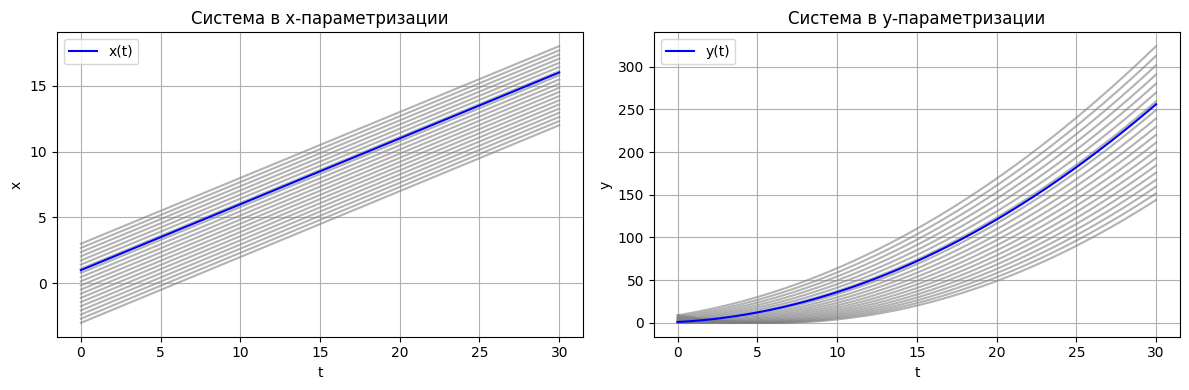
\includegraphics[width=1\linewidth]{images/parametrizationdependency}
    \caption{Интегральные кривые при различных начальных условиях.}
\end{figure*}
\end{note}
\begin{example}
    Пусть есть точка, которая может двигаться по прямой в потенциальном поле $\Pi(x) = x^4\sin \dfrac{1}{x^2}$.
    Исследуем положение равновесия $x = 0$ на устойчивость. \\
    Зафиксируем некоторое $\epsilon > 0$.
    Поскольку система -- консервативна, то полная энергия системы $T + \Pi$ сохраняется и в $B_{\delta}(0)$ выполняется
    \[
        T + \Pi \leq \dfrac{\delta^2}{2} + \delta^4.
    \]
    В то же время, потенциал не может стать слишком большим: $|\Pi| \leq (\epsilon^*)^4$, где $\epsilon^*$~---~положение первого максимума справа от $T + \Pi$.
    Тогда, для зафиксированого $\epsilon > 0$ мы можем подобрать $\epsilon^*$ слева и, таким образом, система не выйдет за пределы $B_{\epsilon^*}(0)$, а, следовательно, и за $B_{\epsilon}(0)$ -- а значит положение равновесия системы устойчиво.
\end{example}
Теперь рассмотрим некоторые эквивалентные определения положений равновесия голономных систем с идеальными связями.
\begin{reminder}
 Будем называть \textit{виртуальным перемещением} механической системы (изохронный дифференциал):
\[
\delta \bt{R} = \sum_{i=1}^N \frac{\partial \bt{R}(\bt{q}, t)}{\partial q_i} \delta q_i
\]
Где положение механической системы задаётся функцией $R$:
\[
\bt{R} = \begin{pmatrix}
\bt{r}_1 \\
\vdots \\
\bt{r}_N
\end{pmatrix},
\]
где $N$ -- количество материальных точек в системе, а $\bt{r_i}$ -- радиус-вектор $i$-ой материальной точки.
\end{reminder}
\begin{theorem}[Принцип виртуальных перемещений]
    Для голономной механической системы с идеальными связями следующие условия эквивалентны:
    \begin{enumerate}
        \item $\bt{R} = \bt{R}^0$~---~положение равновесия.
        \item Работа активных сил на любых виртуальных перемещениях из $\bt{q}^0$ равна 0.
    \end{enumerate}
\end{theorem}
\begin{proof}
    Импликация $1) \Ra 2)$ очевидна в силу основного уравнения динамики:
    \[
        \sum\limits_j (\bt{F}_j - m_j \ddot{\bt{r}_j})\delta \bt{r}_j = 0.
    \]
    И действительно: если $\bt{R} = \bt{R}^0$~---~положение равновесия, то $\forall j = \overline{1, N} \hookrightarrow \ddot{\bt{r}_j} = 0$, а значит
    \[
        \sum\limits_j \bt{F}_j \delta \bt{r}_j = 0.
    \]
    И работа на всяких виртуальных перемещениях действительно равна нулю. \\
    Докажем тепепь $2) \Ra 1)$.
    Поскольку работа активных сил на любых виртуальных перемещениях равна нулю, то
    \[
        \sum\limits_j m_j \ddot{\bt{r}_j} \delta \bt{r}_j = 0.
    \]
    А значит $\forall j \hookrightarrow  \ddot{\bt{r}_j} = 0$.
    Но тогда рассматриваемое положение является положением равновесия и теорема доказана.
\end{proof}

\begin{reminder}
Обобщённой силой, соответствующей обобщённой координате \( q_i \), называется величина
\[
Q_i = \sum_{j=1}^N \bt{F}_j \cdot \frac{\partial \bt{r}_j}{\partial q_i},
\]
где \( \bt{F}_j \) — активная сила, действующая на \( j \)-ю материальную точку, \( \bt{r}_j \) — её радиус-вектор, а \( q_i \) — обобщённая координата.

\end{reminder}

\begin{theorem}
    Пусть есть некоторая голономная механическая система, параметризованная обобщёнными координатами $\bt{q}$.
    Тогда следующие условия эквивалентны:
    \begin{enumerate}
        \item $\bt{q} = \bt{q}^0$ является положением равновесия.
        \item $\bt{Q} = \bt{0}$, где $\bt{Q}$~---~вектор обобщённых сил в этой точке.
    \end{enumerate}
\end{theorem}
\begin{proof}
    Поскольку виртуальные перемещения выражаются как
    \[
        \delta \bt{r}_j = \dfrac{\partial \bt{r}_j}{\partial \bt{q}}\delta \bt{q}.
    \]
    А обобщённые силы равны
    \[
        \bt{Q} = \sum\limits_{j} \bt{F}_j \dfrac{\partial \bt{r}_j}{\partial \bt{q}}.
    \]
    Таким образом утверждение теоремы есть не более чем переформулировка предыдущей теоремы и доказано ранее.
\end{proof}
\begin{note}
    Нетрудно заметить что для консервативных систем равновесия являются стационарными точками потенциала, поскольку $\bt{Q} = -\dfrac{\partial \Pi}{\partial \bt{q}}$.
\end{note}